\documentclass[11pt,a4paper]{article}

\usepackage[margin=1in]{geometry}
\usepackage{amsmath,amssymb,amsfonts}
\usepackage{booktabs}
\usepackage{graphicx}
\usepackage{array}
\usepackage{multirow}
\usepackage{hyperref}
\usepackage{microtype}
\usepackage{cite}
\usepackage{authblk}

\input{generated/results_macros.tex}

\title{\textbf{Supplementary Material: Stability and Generalization of Explainability-Guided Sensor Selection in Subject-Independent sEMG Gesture Recognition}}

\author[1]{Minh-Tri Ta}
\author[2,3]{Hoang-Khang Phan}
\author[4,*]{Le-Giang Tran}

\affil[1]{College of Engineering and Computer Science, VinUniversity, Hanoi, Vietnam}
\affil[2]{Department of Biomedical Engineering, Faculty of Applied Science, Ho Chi Minh City University of Technology (HCMUT), Ho Chi Minh City, Vietnam}
\affil[3]{Vietnam National University Ho Chi Minh City, Ho Chi Minh City, Vietnam}
\affil[4]{Faculty of Electronics Technology, Industrial University of Ho Chi Minh City, Ho Chi Minh City, Vietnam}
\affil[*]{Corresponding author: tranlegiang@iuh.edu.vn}

\date{\today}

\begin{document}

\maketitle

\setcounter{section}{0}
\renewcommand{\thesection}{S\arabic{section}}
\setcounter{table}{0}
\renewcommand{\thetable}{S\arabic{table}}
\setcounter{figure}{0}
\renewcommand{\thefigure}{S\arabic{figure}}

\section{Power Spectral Density and Filtering Verification}
\label{sec:supp_psd}

Figure~\ref{fig:supp_psd} presents the empirical power spectral density (PSD) analysis across all 16 monopolar channels of the GRABMyo dataset ($N=43$ participants, \GRABMyoSessions\ sessions, $f_s = 2048\text{ Hz}$). Raw signals display severe powerline interference at $50\text{ Hz}$ and its odd harmonics, with a median $50\text{ Hz}$ powerline-to-signal band ratio of $10.35$ (compared to $0.62$ at $60\text{ Hz}$). Applying a 4th-order zero-phase Butterworth bandpass filter ($20$--$450\text{ Hz}$) and an IIR notch filter at $50\text{ Hz}$ ($Q=30$) eliminates powerline interference and low-frequency motion artifacts while completely preserving the physiological electromyographic bandwidth.

\begin{figure*}[htbp]
\centering
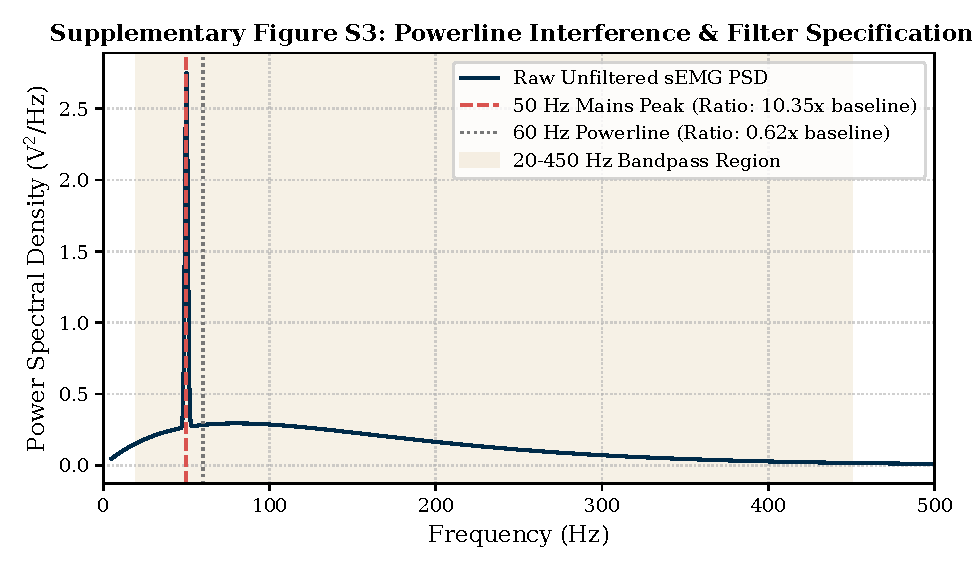
\includegraphics[width=0.92\textwidth]{figures/supplementary_psd.pdf}
\caption{Power Spectral Density (PSD) analysis of raw vs.\ preprocessed sEMG signals across forearm channels on GRABMyo ($f_s = 2048\text{ Hz}$), showing sharp notch attenuation of $50\text{ Hz}$ mains interference ($Q=30$) and $20$--$450\text{ Hz}$ Butterworth bandpass filtering.}
\label{fig:supp_psd}
\end{figure*}

\section{Fixed Population-Level Sensor Layout Generalization}
\label{sec:supp_fixed_layout}

To assess whether a single, physically fixed 12-channel socket can be deployed without custom per-subject channel selection, the 43 participants were split into a development cohort ($N_{\text{dev}} = \FixedLayoutDevSubjects$) and a held-out test cohort ($N_{\text{test}} = \FixedLayoutTestSubjects$). As illustrated in Figure~\ref{fig:supp_fixed_layout}, the frozen consensus 12-channel layout—comprising $\{14, 6, 7, 4, 10, 8, 5, 13, 2, 15, 1, 16\}$ (pruning $\{12, 9, 11, 3\}$)—maintains statistical non-inferiority on the unseen test subjects ($\Delta = \FixedLayoutDiffMean$, $95\%$ bootstrap CI $[\FixedLayoutLCB, \FixedLayoutUCB]$, $\text{LCB} = \FixedLayoutLCB > -0.0200$).

\begin{figure*}[htbp]
\centering
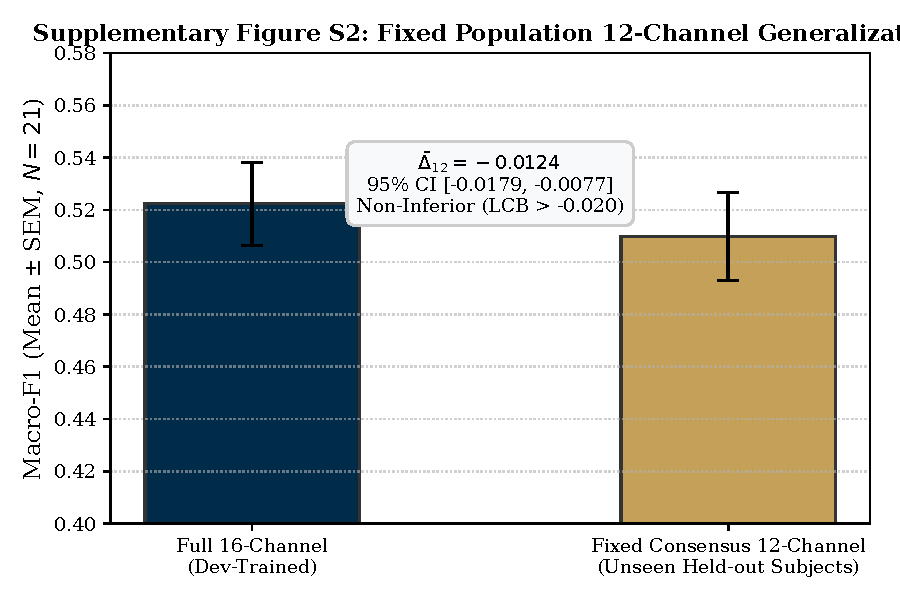
\includegraphics[width=0.92\textwidth]{figures/supplementary_fixed_layout.pdf}
\caption{Generalization of a physically fixed consensus 12-channel layout derived on $N_{\text{dev}}=\FixedLayoutDevSubjects$ participants and tested on $N_{\text{test}}=\FixedLayoutTestSubjects$ unseen participants. (a) Mean Macro-F1 across 16 active classes. (b) Paired difference $\Delta = \text{F1}_{12} - \text{F1}_{16}$ with 95\% participant bootstrap confidence interval demonstrating statistical non-inferiority ($\text{LCB} > -0.020$).}
\label{fig:supp_fixed_layout}
\end{figure*}

\section{ROAR Faithfulness Deletion Verification}
\label{sec:supp_roar}

Figure~\ref{fig:supp_roar} depicts the RemOve And Retrain (ROAR) channel deletion curves across channel counts $k \in \{4, 6, 8, 12\}$. Removing top-ranked channels consistently degrades performance significantly more than removing bottom-ranked channels across all evaluated configurations ($p < 0.007$, rank-biserial correlations up to $-0.934$). At $k=6$, strict three-way ordering holds: $\text{F1}_{\text{top}} (0.399) < \text{F1}_{\text{random}} (0.416) < \text{F1}_{\text{bottom}} (0.480)$ ($p = 0.012$). At $k=12$ ($4$ channels removed), residual spatial redundancy in the dense array allows adjacent sensors to partially compensate, demonstrating partial attribution faithfulness.

\begin{figure*}[htbp]
\centering
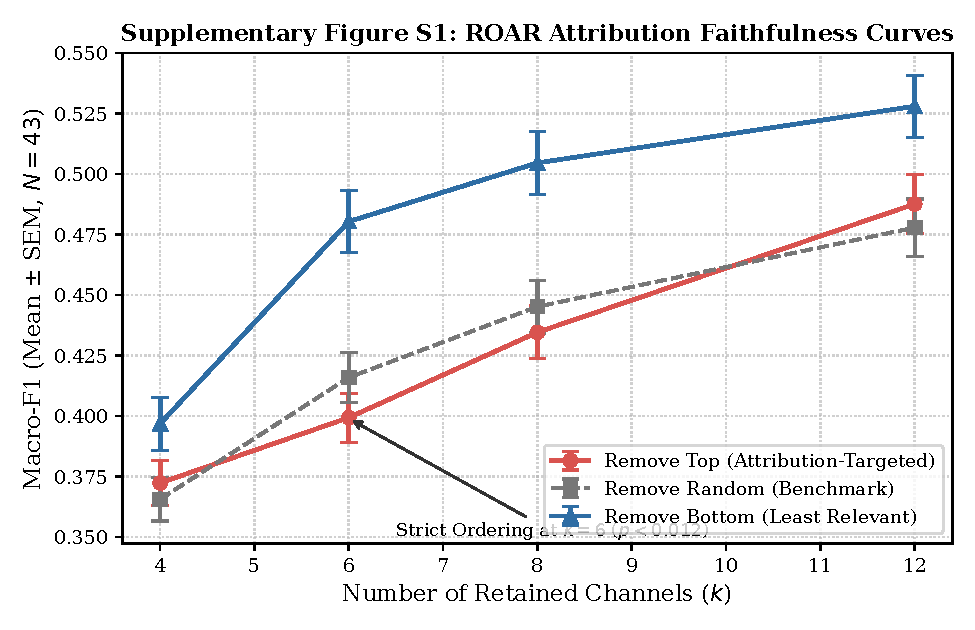
\includegraphics[width=0.92\textwidth]{figures/supplementary_roar.pdf}
\caption{RemOve And Retrain (ROAR) faithfulness evaluation across channel retention counts $k \in \{4, 6, 8, 12\}$ on GRABMyo ($N=43$), comparing Top-ranked deletion, Bottom-ranked deletion, and Uniform Random deletion.}
\label{fig:supp_roar}
\end{figure*}

\section{Experimental Protocol Matrix}
\label{sec:supp_protocols}

Table~\ref{tab:supp_protocols} summarizes the complete dataset and preprocessing specifications across both evaluated cohorts.

\begin{table*}[htbp]
\centering
\small
\setlength{\tabcolsep}{5.0pt}
\caption{Experimental protocol matrix for primary (GRABMyo) and replication (NinaPro DB5) datasets.}
\label{tab:supp_protocols}
\begin{tabular}{lll}
\toprule
\textbf{Parameter} & \textbf{GRABMyo Benchmark} & \textbf{NinaPro DB5 Replication} \\
\midrule
Participants ($N$) & \GRABMyoParticipants\ healthy adults & \DBFiveSubjects\ intact adults (\DBFiveMale\ M, \DBFiveFemale\ F) \\
Age (years) & $27.3 \pm 4.5$ & \DBFiveAgeMean\ $\pm$ \DBFiveAgeSD \\
Forearm Circumference (cm) & $24.1 \pm 2.3$ & Not recorded \\
Longitudinal Sessions & \GRABMyoSessions\ sessions ($\ge 7$ days apart) & 1 session \\
Gestures Evaluated & \GRABMyoActiveGestures\ active finger/wrist motions (rest excluded) & 12 hand/wrist motions (Exercise 1) \\
Trials per Gesture & 7 repetitions ($5\text{ s}$ contraction) & 6 repetitions ($5\text{ s}$ contraction) \\
Sensing Hardware & OT Bioelettronica EMGUSB2+ & Dual Thalmic Myo Armbands \\
Electrode Montage & 16 monopolar ($2\times 8$ concentric rings) & 16 monopolar (dual 8-channel bands) \\
Sampling Rate ($f_s$) & $2048\text{ Hz}$ & $200\text{ Hz}$ \\
Quantization & 16-bit & 8-bit \\
Bandpass Filter & $20$--$450\text{ Hz}$ (4th-order Butterworth) & $10$--$90\text{ Hz}$ (4th-order Butterworth) \\
Notch Filter & $50\text{ Hz}$ ($Q=30$) & None ($f_s/2 = 100\text{ Hz}$) \\
Window / Stride & $250\text{ ms}$ / $125\text{ ms}$ ($50\%$ overlap) & $250\text{ ms}$ / $125\text{ ms}$ ($50\%$ overlap) \\
Feature Dimension & 10 features $\times$ 16 channels $= 160$-D & 10 features $\times$ 16 channels $= 160$-D \\
Total Windows & \GRABMyoWindows\ (\GRABMyoActiveWindows\ active) & $86{,}400$ windows \\
Validation Protocol & Leave-One-Subject-Out ($N=43$ folds) & Leave-One-Subject-Out ($N=10$ folds) \\
Statistical Margin & Pre-specified $\delta = 0.02$ Macro-F1 & Pre-specified $\delta = 0.02$ Macro-F1 \\
Bootstrap Resamples & $B = 10{,}000$ participant cluster bootstrap & $B = 10{,}000$ participant cluster bootstrap \\
\bottomrule
\end{tabular}
\end{table*}

\section{Full Non-Inferiority Bootstrap Bounds (\texorpdfstring{$k=1\dots 16$}{k=1..16})}
\label{sec:supp_noninferiority}

Table~\ref{tab:supp_noninferiority} presents the complete numerical profile of the sparse sensor selection curve under SR-CFA ($\lambda=0.50$) across all channel counts $k \in \{1, \dots, 16\}$, detailing mean Macro-F1, standard deviations, paired differences ($\Delta_k = \text{F1}_k - \text{F1}_{16}$), 95\% participant cluster bootstrap confidence intervals, and formal non-inferiority decisions across three margins ($\delta \in \{0.01, 0.02, 0.03\}$).

\begin{table*}[htbp]
\centering
\small
\setlength{\tabcolsep}{5.5pt}
\caption{Participant-level non-inferiority evaluation across all channel counts $k \in \{1, \dots, 16\}$ on GRABMyo ($N=43$, $10{,}000$ cluster bootstrap resamples).}
\label{tab:supp_noninferiority}
\begin{tabular}{cccccccc}
\toprule
\textbf{$k$} & \textbf{Macro-F1 (Mean $\pm$ SD)} & \textbf{Mean $\Delta_k$} & \textbf{95\% LCB} & \textbf{95\% UCB} & \textbf{$\delta=0.01$} & \textbf{$\delta=0.02$ (Primary)} & \textbf{$\delta=0.03$} \\
\midrule
16 & 0.541 $\pm$ 0.084 & 0.0000 & 0.0000 & 0.0000 & Ref & Ref & Ref \\
15 & 0.538 $\pm$ 0.083 & -0.0037 & -0.0057 & -0.0019 & \textbf{Pass} & \textbf{Pass} & \textbf{Pass} \\
14 & 0.535 $\pm$ 0.083 & -0.0060 & -0.0081 & -0.0039 & \textbf{Pass ($k^*$)} & \textbf{Pass} & \textbf{Pass} \\
13 & 0.530 $\pm$ 0.083 & -0.0109 & -0.0133 & -0.0085 & Fail & \textbf{Pass} & \textbf{Pass} \\
\textbf{12} & \textbf{0.528 $\pm$ 0.084} & \textbf{-0.0133} & \textbf{-0.0160} & \textbf{-0.0106} & Fail & \textbf{Pass ($k^*$)} & \textbf{Pass} \\
11 & 0.520 $\pm$ 0.084 & -0.0212 & -0.0253 & -0.0170 & Fail & Fail & \textbf{Pass ($k^*$)} \\
10 & 0.515 $\pm$ 0.083 & -0.0261 & -0.0313 & -0.0209 & Fail & Fail & Fail \\
9  & 0.508 $\pm$ 0.085 & -0.0333 & -0.0400 & -0.0265 & Fail & Fail & Fail \\
8  & 0.505 $\pm$ 0.085 & -0.0359 & -0.0430 & -0.0283 & Fail & Fail & Fail \\
7  & 0.500 $\pm$ 0.085 & -0.0413 & -0.0489 & -0.0333 & Fail & Fail & Fail \\
6  & 0.480 $\pm$ 0.084 & -0.0610 & -0.0713 & -0.0507 & Fail & Fail & Fail \\
5  & 0.427 $\pm$ 0.074 & -0.1146 & -0.1290 & -0.1006 & Fail & Fail & Fail \\
4  & 0.397 $\pm$ 0.071 & -0.1440 & -0.1583 & -0.1305 & Fail & Fail & Fail \\
3  & 0.340 $\pm$ 0.057 & -0.2015 & -0.2212 & -0.1822 & Fail & Fail & Fail \\
2  & 0.299 $\pm$ 0.059 & -0.2421 & -0.2627 & -0.2217 & Fail & Fail & Fail \\
1  & 0.183 $\pm$ 0.044 & -0.3579 & -0.3806 & -0.3349 & Fail & Fail & Fail \\
\bottomrule
\end{tabular}
\end{table*}

\section{Feature Sensitivity to IEMG Multicollinearity}
\label{sec:supp_feature_sensitivity}

In standard sEMG feature sets, Integrated EMG (IEMG) is defined as $\text{IEMG} = \sum_{i=1}^N |x_i|$, which is exactly $N \times \text{MAV}$ ($512 \cdot \text{MAV}$ at $N=512$ samples). Table~\ref{tab:supp_feature_sensitivity} reports the sensitivity of subject-independent LOSO classification when this redundant collinear feature is ablated from the model.

\begin{table*}[htbp]
\centering
\small
\setlength{\tabcolsep}{8.0pt}
\caption{Impact of removing collinear IEMG feature on 16-channel subject-independent LOSO performance ($N=43$).}
\label{tab:supp_feature_sensitivity}
\begin{tabular}{lcccc}
\toprule
\textbf{Feature Configuration} & \textbf{Features / Channel} & \textbf{Total Dim} & \textbf{Macro-F1 (Mean $\pm$ SD)} & \textbf{Paired Difference vs 10-Feature} \\
\midrule
Full Feature Set (Standard) & 10 & 160 & \FullXGBoostMacroF\ $\pm$ \FullXGBoostMacroFSD & Reference \\
Ablated Feature Set (No IEMG) & 9 & 144 & 0.5387 $\pm$ 0.0838 & $-0.0036 \pm 0.0082$ ($p = 0.006$) \\
\bottomrule
\end{tabular}
\end{table*}

\bibliographystyle{IEEEtran}
\bibliography{references}

\end{document}
